\documentclass[11pt,a4paper]{article}

% ==============================================================================
% PACKAGES & CONFIGURATION
% ==============================================================================
\usepackage[utf8]{inputenc}
\usepackage[T1]{fontenc}
\usepackage[margin=1in]{geometry}
\usepackage{amsmath,amssymb,amsfonts,bm}
\usepackage{booktabs,multirow,array}
\usepackage{graphicx}
\usepackage{xcolor}
\usepackage{tikz}
\usetikzlibrary{shapes.geometric, arrows.meta, positioning, calc, fit, backgrounds}
\usepackage{pgfplots}
\pgfplotsset{compat=1.18}
\usepackage{caption}
\usepackage{subcaption}
\usepackage{float}
\usepackage{listings}
\usepackage{lmodern}
\usepackage{enumitem}
\usepackage[protrusion=true,expansion=false]{microtype}
\usepackage{cite}
\usepackage[colorlinks=true, linkcolor=kuetblue, citecolor=kuetblue, urlcolor=kuetblue]{hyperref}

% Color definitions
\definecolor{kuetblue}{RGB}{0, 51, 102}
\definecolor{kuetgold}{RGB}{184, 134, 11}
\definecolor{cardbg}{RGB}{248, 250, 252}
\definecolor{bordergray}{RGB}{220, 226, 235}
\definecolor{darkgray}{RGB}{50, 50, 50}
\definecolor{codegreen}{RGB}{46, 139, 87}
\definecolor{codered}{RGB}{178, 34, 34}

% Listings setup
\lstset{
	basicstyle=\ttfamily\footnotesize,
	breaklines=true,
	frame=single,
	backgroundcolor=\color{cardbg},
	rulecolor=\color{bordergray},
	keywordstyle=\color{kuetblue}\bfseries,
	commentstyle=\color{codegreen}\itshape,
	stringstyle=\color{codered},
	showstringspaces=false
}

% Section formatting
\usepackage{titlesec}
\titleformat{\section}{\color{kuetblue}\large\bfseries}{\thesection.}{0.6em}{}
\titleformat{\subsection}{\color{kuetblue}\normalsize\bfseries}{\thesubsection.}{0.5em}{}
\titleformat{\subsubsection}{\color{darkgray}\normalsize\bfseries}{\thesubsubsection.}{0.5em}{}

% Header and Footer (Top Header and rule removed; centered page number retained)
\usepackage{fancyhdr}
\pagestyle{fancy}
\fancyhf{}
\renewcommand{\headrulewidth}{0pt}
\renewcommand{\footrulewidth}{0pt}
\fancyfoot[C]{\thepage}

% Float parameters for tight, professional visual density
\renewcommand{\topfraction}{0.90}
\renewcommand{\bottomfraction}{0.90}
\renewcommand{\textfraction}{0.10}
\renewcommand{\floatpagefraction}{0.85}
\setlength{\floatsep}{8pt plus 2pt minus 2pt}
\setlength{\textfloatsep}{10pt plus 2pt minus 2pt}
\setlength{\intextsep}{8pt plus 2pt minus 2pt}
\setlength{\abovecaptionskip}{4pt plus 1pt minus 1pt}
\setlength{\belowcaptionskip}{4pt plus 1pt minus 1pt}

% ==============================================================================
% FORMAL ALGORITHM ENVIRONMENT DEFINITION (STRICT IN-LINE PLACEMENT [H])
% ==============================================================================
\newcounter{algfloat}
\renewcommand{\thealgfloat}{\arabic{algfloat}}
\newcounter{algline}[algfloat]
\newcommand{\algstep}{\stepcounter{algline}\par\noindent\makebox[2.2em][r]{\footnotesize\color{darkgray}\thealgline:\hspace{0.6em}}}
\newcommand{\algindent}[1]{\stepcounter{algline}\par\noindent\makebox[2.2em][r]{\footnotesize\color{darkgray}\thealgline:\hspace{0.6em}}\hspace*{#1\dimexpr 1.25em\relax}}

\newenvironment{formalalgorithm}[2][H]{%
	\refstepcounter{algfloat}%
	\begin{figure}[#1]%
		\centering
		\begin{minipage}{0.96\linewidth}
			\hrule height 0.9pt depth 0pt\kern 4pt
			\noindent\textbf{Algorithm \thealgfloat:} #2\par
			\kern 3pt\hrule height 0.4pt depth 0pt\kern 6pt
			\footnotesize
		}{%
			\par\kern 6pt\hrule height 0.9pt depth 0pt
		\end{minipage}
	\end{figure}
}

% ==============================================================================
% DOCUMENT BEGIN
% ==============================================================================
\begin{document}
	
	% ==============================================================================
	% TITLE PAGE / METADATA HEADER
	% ==============================================================================
	\begin{titlepage}
		\centering
		\vspace*{0.3cm}
		
		{\Large \textbf{KHULNA UNIVERSITY OF ENGINEERING \& TECHNOLOGY (KUET)}}\\[0.25cm]
		{\large Department of Computer Science and Engineering}\\[0.15cm]
		{\normalsize Khulna--9203, Bangladesh}\\[0.7cm]
		
		\rule{\linewidth}{1.2pt}\\[0.4cm]
		{\Large \bfseries \color{kuetblue} News Category Classification and Semantic Analysis Using Traditional NLP Methods}\\[0.3cm]
		\rule{\linewidth}{1.2pt}\\[0.6cm]
		
		{\large \textbf{Course Title:} Natural Language Processing Laboratory}\\[0.15cm]
		{\large \textbf{Course Code:} CSE 4122}\\[0.15cm]
		{\normalsize Academic Session: 2024--2025 (4th Year, 1st Term)}\\[1.0cm]
		
		\begin{minipage}[t]{0.48\textwidth}
			\flushleft
			\vspace{1.5cm}
			\textbf{\large Submitted By:}\\[0.2cm]
			\textbf{Adnan Hossain Siraz}\\
			Roll No.: 2107068\\
			Department of CSE, KUET\\[0.5cm]
			
			\textbf{Md. Shakibuzzaman}\\
			Roll No.: 2107069\\
			Department of CSE, KUET
		\end{minipage}
		\hfill
		\begin{minipage}[t]{0.48\textwidth}
			\flushright
			\vspace{1.5cm}
			\textbf{\large Supervised By:}\\[0.2cm]
			\textbf{Dr. K. M. Azharul Hasan}\\
			Professor, Department of CSE\\
			Khulna University of Engineering \& Technology\\[0.4cm]
			\textbf{Mr. Md. Nazirulhasan Shawon}\\
			Lecturer, Department of CSE\\
			Khulna University of Engineering \& Technology
		\end{minipage}
		
		\vfill
		{\large \textbf{Date of Submission:} 23 September 2026}\\[0.2cm]
		\rule{0.4\linewidth}{0.5pt}\\
		
	\end{titlepage}
	
	\newpage
	\pagenumbering{arabic}
	
	% ==============================================================================
	% SECTION 1: INTRODUCTION
	% ==============================================================================
	\section{Introduction}
	\label{sec:introduction}
	
	Automated topic categorization of unstructured news text represents an essential foundational pillar in computational linguistics, modern information retrieval, and algorithmic content recommendation engines \cite{manning2008introduction}. As digital media platforms produce massive volumes of journalistic reporting daily, categorizing continuous news streams into discrete semantic buckets---such as \textit{Business}, \textit{Entertainment}, \textit{Politics}, \textit{Sport}, and \textit{Technology}---is critical for efficient retrieval, trending topic detection, and personalized user consumption[cite: 3, 6]. In academic research and industrial engineering alike, the design of text representation pipelines dictates both the upper bound on classification accuracy and the system's operational viability under stringent latency and hardware constraints[cite: 4, 6].
	
	\subsection{Problem Statement \& Linguistic Dynamics}
	While document-level classification for long-form journalistic articles is well-established, severe degradation in classification performance occurs when traditional models encounter \textit{short-form text} (e.g., news headlines, breaking news tickers, social micro-posts, and push notifications) \cite{wang2012baselines}. Long-form news documents typically contain 200 to 800 words, offering dense repetition of thematic keywords and broad vocabulary distributions that yield reliable document frequencies[cite: 3, 6]. Conversely, short-form headlines consist of only 4 to 12 words[cite: 3, 6]. In such constrained inputs, standard bag-of-words (BoW) representations suffer from extreme mathematical sparsity, acute out-of-vocabulary (OOV) rates, and severe vulnerability to polysemous term overlap[cite: 3, 6].
	
	A central linguistic phenomenon observed during practical evaluation is \textit{semantic shift} and cross-domain lexical borrowing[cite: 6]. In authentic news corpora, vocabulary terms are not strictly partitioned among categories[cite: 3, 6]. For example, financial and commercial terminology frequently appears in sports reporting (e.g., player transfers, franchise buyouts, stadium sponsorship debt, club administration), while geopolitical terms routinely dominate economic coverage (e.g., bilateral trade tariffs, ministerial declarations, sovereign borrowing)[cite: 3, 6]. Under dense vector averaging, short texts lacking explicit domain-exclusive nouns frequently experience representation collapse toward the corpus's dominant lexical distribution[cite: 3, 6].
	
	\subsection{Theoretical Representation Paradigms}
	Text categorization fundamentally depends on transforming variable-length sequences of discrete lexical tokens into vector representations suitable for statistical optimization[cite: 4, 6]. Historically, two competing paradigms have dominated traditional natural language processing[cite: 4, 6]:
	\begin{enumerate}[leftmargin=1.5em, itemsep=0.2em]
		\item \textbf{High-Dimensional Sparse Frequency Models:} Methods such as Term Frequency--Inverse Document Frequency ($\text{TF-IDF}$) map documents into high-dimensional vector spaces ($V \sim 10^3$--$10^5$), where each dimension corresponds to an exact unigram or higher-order n-gram[cite: 4, 6]. While these representations excel at capturing exact domain keywords and phrases without semantic blurring, they inherently suffer from orthogonal basis independence: synonyms (e.g., \textit{``equity''} and \textit{``stock''}) share zero inner-product overlap[cite: 4, 6].
		\item \textbf{Continuous Distributed Latent Manifolds:} Continuous embedding techniques, pioneered by Word2Vec \cite{mikolov2013distributed}, map words to low-dimensional continuous vector spaces ($\mathbb{R}^d$, where $d \sim 50$--$300$) where cosine distance captures semantic similarity[cite: 4, 6]. When pooling word embeddings into a unified document vector, however, standard unweighted averaging causes \textit{centroid dilution}: ubiquitous and polysemous words distort the document centroid, pulling the resulting vector away from decisive thematic markers[cite: 4, 6].
	\end{enumerate}
	
	\subsection{Core Objectives \& Contributions}
	This research project delivers a rigorous, formula-first comparative investigation of frequency-based sparse representations and dense semantic vector spaces for multi-class news categorization[cite: 3, 6]. Developed strictly from foundational mathematical equations without black-box library wrappers, this work provides[cite: 4, 6]:
	\begin{itemize}[leftmargin=1.5em, itemsep=0.2em]
		\item \textbf{Traditional NLP Classification:} Implementation and comparison of Multinomial Naive Bayes and One-vs-Rest Logistic Regression using multiple classical text representations[cite: 6].
		\item \textbf{Multiple Text Representations:} Evaluation of Bag-of-Words, TF-IDF unigram/bigram features, custom Skip-Gram Word2Vec document vectors, and pretrained GloVe document vectors[cite: 6].
		\item \textbf{Zero-Leakage Feature Construction:} Vocabulary, document frequency, and inverse document frequency statistics are learned from the training partition and then applied unchanged to the held-out test set[cite: 6].
		\item \textbf{Semantic Analysis:} Use of Word2Vec/GloVe embeddings and cosine similarity to explore relationships between words in a continuous vector space[cite: 6].
		\item \textbf{Seven-Pipeline Benchmark:} Systematic comparison of seven traditional NLP classification pipelines on the 2,225-document, five-category BBC News dataset using a fixed 445-document held-out test set[cite: 6].
		\item \textbf{Error Analysis and Explainability:} Investigation of representative classification errors, including the short sports headline \textit{``brazil lost 7-1 against germany''}, together with linear feature attribution in the interactive interface[cite: 6].
		\item \textbf{Interactive Demonstration:} Development of an offline Streamlit dashboard for live classification, semantic exploration, and benchmark inspection[cite: 6].
	\end{itemize}
	
	% ==============================================================================
	% SECTION 2: BACKGROUND AND THEORETICAL FORMULATIONS
	% ==============================================================================
	\section{Background and Theoretical Formulations}
	\label{sec:background}
	
	This section establishes the mathematical foundations, governing equations, and optimization objectives underpinning the feature extractors, embedding aggregators, and linear classification heads implemented in this work[cite: 4, 6].
	
	\subsection{Term Frequency--Inverse Document Frequency (\texorpdfstring{$\text{TF-IDF}$}{TF-IDF})}
	Frequency-based text representation models map unstructured token sequences into a vector space $\mathbb{R}^V$, where $V$ represents the pre-defined vocabulary size[cite: 4, 6]. Raw term frequencies are scaled by their inverse document frequency to discount universally ubiquitous words while elevating domain-discriminative terms \cite{salton1988term}.
	
	Let $f_{t, d}$ denote the raw occurrence count of term $t$ in document $d$[cite: 3, 6]. The normalized term frequency is defined as[cite: 3, 6]:
	\begin{equation}
		\text{TF}(t, d) = \frac{f_{t, d}}{\sum_{t' \in d} f_{t', d}}
		\label{eq:tf}
	\end{equation}
	To prevent division-by-zero singularities and dampen logarithmic scale distortion on finite training collections, we implement the smoothed inverse document frequency[cite: 3, 6]:
	\begin{equation}
		\text{IDF}(t) = \ln\left(\frac{N_{\text{train}} + 1}{\text{DF}_{\text{train}}(t) + 1}\right) + 1
		\label{eq:idf}
	\end{equation}
	where $N_{\text{train}}$ denotes the total number of articles in the training partition, and $\text{DF}_{\text{train}}(t)$ represents the number of training articles containing term $t$[cite: 3, 6]. The unnormalized feature value is $v_d[j] = \text{TF}(t_j, d) \times \text{IDF}(t_j)$[cite: 3, 6]. To eliminate document length bias, the vector is normalized under the Euclidean $L_2$ norm[cite: 3, 6]:
	\begin{equation}
		x_d = \frac{v_d}{\|v_d\|_2} = \frac{v_d}{\sqrt{\sum_{j=1}^{V} (v_d[j])^2}}
		\label{eq:l2_norm}
	\end{equation}
	
	\subsection{Word2Vec: Skip-Gram with Negative Sampling (SGNS)}
	While $\text{TF-IDF}$ captures global document-level statistics, it inherently treats vocabulary terms as orthogonal basis vectors, discarding semantic synonymy and context-dependent relationships[cite: 3, 6]. Distributed representations map tokens into a continuous low-dimensional latent manifold $\mathbb{R}^d$ ($d \ll V$) such that words sharing similar distributional contexts occupy proximal coordinates \cite{mikolov2013distributed}.
	
	In the Skip-Gram architecture, given a sequence of training tokens $w_1, w_2, \dots, w_T$, the model maximizes the average log probability of predicting context words within a sliding window of radius $c$ centered at target token $w_t$[cite: 3, 6]:
	\begin{equation}
		\mathcal{L}_{\text{SG}} = \frac{1}{T} \sum_{t=1}^{T} \sum_{-c \le j \le c, j \ne 0} \log P(w_{t+j} \mid w_t)
		\label{eq:sg_obj}
	\end{equation}
	Because computing exact full-vocabulary softmax normalization is computationally intractable ($\mathcal{O}(|V|)$ per gradient step), we utilize Negative Sampling (SGNS)[cite: 4, 6]. SGNS reformulates context prediction into binary logistic regressions differentiating true observed context pairs from $K$ noise samples[cite: 4, 6]:
	\begin{equation}
		\mathcal{L}_{\text{SGNS}} = \sum_{t=1}^{T} \sum_{-c \le j \le c, j \ne 0} \left[ \log \sigma\left({v'_{w_{t+j}}}^\top v_{w_t}\right) + \sum_{k=1}^{K} \mathbb{E}_{w_{n,k} \sim P_n(w)} \left[ \log \sigma\left(-{v'_{w_{n,k}}}^\top v_{w_t}\right) \right] \right]
		\label{eq:sgns_loss}
	\end{equation}
	where $v_w, v'_w \in \mathbb{R}^d$ represent target and context embeddings, and $\sigma(z) = \frac{1}{1 + e^{-z}}$ is the logistic sigmoid activation[cite: 4, 6].
	
	The negative noise samples are drawn from the smoothed unigram distribution $P_n(w) \propto f(w)^{3/4}$[cite: 4, 6]. This sub-linear scaling dampens ubiquitous stopwords while elevating the sampling probability of rare and domain-specific terms, ensuring sufficient negative gradient signal without destabilizing parameter updates[cite: 4, 6].
	
	\subsection{Document Vector Aggregation: Naive vs. Weighted Centroid}
	Because Word2Vec models produce token-level vectors $v_w$, an aggregation mechanism is required to map variable-length documents $d = \{w_1, w_2, \dots, w_{|d|}\}$ into a fixed-dimensional document embedding $v_d \in \mathbb{R}^d$[cite: 3, 6].
	
	\subsubsection{Arithmetic Mean Pooling}
	The standard baseline computes the unweighted centroid across all in-vocabulary tokens[cite: 3, 6]:
	\begin{equation}
		v_d^{\text{mean}} = \frac{1}{|d \cap \mathcal{V}|} \sum_{w \in d \cap \mathcal{V}} v_w
		\label{eq:mean_pooling}
	\end{equation}
	A critical theoretical failure of arithmetic mean pooling is that ubiquitous, generic vocabulary terms exert equal gravitational pull on the centroid as highly specific topical markers, diluting class-discriminative signals[cite: 3, 6].
	
	\subsubsection{TF-IDF Weighted Centroid Aggregation}
	To suppress common semantic drift, we weight each token vector by its precomputed training $\text{TF-IDF}$ significance[cite: 3, 6]:
	\begin{equation}
		v_d^{\text{tfidf}} = \frac{\sum_{w \in d \cap \mathcal{V}} \text{TF-IDF}(w, d) \cdot v_w}{\sum_{w \in d \cap \mathcal{V}} \text{TF-IDF}(w, d)}
		\label{eq:tfidf_pooling}
	\end{equation}
	If all words in document $d$ are out-of-vocabulary ($d \cap \mathcal{V} = \emptyset$), $v_d$ defaults to the zero vector $\mathbf{0}_d$, prompting the linear classifier to default gracefully to empirical class prior distributions[cite: 3, 6].
	
	\subsection{Multinomial Logistic Regression Formulation}
	For multi-class classification across $C = 5$ categories with feature vector $x \in \mathbb{R}^p$, the linear logits are $z = W x + b$, where $W \in \mathbb{R}^{C \times p}$ and $b \in \mathbb{R}^C$[cite: 4, 6]. The posterior class probability distribution is given by the Softmax function[cite: 3, 6]:
	\begin{equation}
		\hat{y}_c = P(y = c \mid x) = \frac{\exp(z_c)}{\sum_{k=1}^{C} \exp(z_k)} = \frac{\exp(w_c^\top x + b_c)}{\sum_{k=1}^{C} \exp(w_k^\top x + b_k)}
		\label{eq:softmax_prob}
	\end{equation}
	Optimization minimizes the regularized categorical cross-entropy loss over $m$ training instances[cite: 3, 6]:
	\begin{equation}
		\mathcal{J}(W, b) = -\frac{1}{m} \sum_{i=1}^{m} \sum_{c=1}^{C} y_{i,c} \log \hat{y}_{i,c} + \frac{\lambda}{2} \sum_{c=1}^{C} \|w_c\|_2^2
		\label{eq:full_cross_entropy}
	\end{equation}
	where $y_{i,c} \in \{0, 1\}$ represents the ground-truth one-hot class label, and $\lambda$ is the $L_2$ Ridge regularization penalty[cite: 4, 6]. Evaluating the gradient with respect to parameters yields the closed-form batch update equation[cite: 4, 6]:
	\begin{equation}
		\nabla_W \mathcal{J} = \frac{1}{m} (\hat{Y} - Y)^\top X + \lambda W, \qquad \nabla_b \mathcal{J} = \frac{1}{m} \sum_{i=1}^{m} (\hat{y}_i - y_i)
		\label{eq:matrix_gradient}
	\end{equation}
	where $X \in \mathbb{R}^{m \times p}$ is the design matrix, $Y \in \mathbb{R}^{m \times C}$ is the one-hot target matrix, and $\hat{Y} \in \mathbb{R}^{m \times C}$ represents predicted softmax posteriors[cite: 4, 6].
	
	\subsection{One-vs-Rest (OvR) Binary Decomposition}
	In the One-vs-Rest decomposition, $C$ independent binary classifiers are trained, each separating category $c$ ($y^{(c)} = 1$) from all remaining classes ($y^{(c)} = 0$)[cite: 4, 6]. Logits are clipped for numerical stability ($z_c \in [-250, 250]$) with sigmoid activation $\hat{p}_c = \sigma(z_c)$[cite: 4, 6]. Parameters are optimized via batch gradient descent with Ridge penalty $\nabla_{w_c} \mathcal{J} = \frac{1}{m} X^\top (\hat{p}_c - y^{(c)}) + \lambda w_c$[cite: 4, 6]. Normalized class probabilities are obtained via $P(y = c \mid x) = \sigma(z_c) / \sum_k \sigma(z_k)$, and linear feature attribution for token $j$ toward category $c$ is given by $\text{Attr}_c(j) = x_d[j] \cdot w_c[j]$[cite: 4, 6].
	
	% ==============================================================================
	% SECTION 3: DATASET, CORPUS, AND PREPROCESSING
	% ==============================================================================
	\section{Dataset, Corpus, and Preprocessing}
	\label{sec:dataset}
	
	\subsection{Corpus Description}
	The experimental investigation is conducted on the official BBC News text classification benchmark, comprising 2,225 authentic journalistic articles published between 2004 and 2005 across five thematic desks[cite: 3, 6]. The corpus contains zero missing values and zero duplicate articles[cite: 3, 6].
	
	\begin{table}[H]
		\centering
		\caption{Dataset distribution across categories and experimental partitions.}
		\label{tab:dataset_split}
		\resizebox{\linewidth}{!}{%
			\begin{tabular}{lcccc}
				\toprule
				\textbf{Category} & \textbf{Total Articles} & \textbf{Proportion (\%)} & \textbf{Train Split ($80\%$)} & \textbf{Held-Out Test ($20\%$)} \\
				\midrule
				Sport         & 511 & 22.97\% & 409 & 102 \\
				Business      & 510 & 22.92\% & 408 & 102 \\
				Politics      & 417 & 18.74\% & 333 & 84  \\
				Tech          & 401 & 18.02\% & 321 & 80  \\
				Entertainment & 386 & 17.35\% & 309 & 77  \\
				\midrule
				\textbf{Total} & \textbf{2,225} & \textbf{100.00\%} & \textbf{1,780} & \textbf{445} \\
				\bottomrule
			\end{tabular}%
		}
	\end{table}
	
	\subsection{Preprocessing Pipeline \& Data Leakage Prevention}
	Text normalization operates through a structured multi-stage pipeline[cite: 3, 6]:
	\begin{enumerate}[leftmargin=1.5em, itemsep=0.2em]
		\item \textbf{HTML and Escaped Character Stripping:} Regular expression cleaning removes residual markup tags and newline formatting artifacts[cite: 3, 6].
		\item \textbf{Case Normalization:} All characters are converted to lowercase[cite: 3, 6].
		\item \textbf{Tokenization Protocols:} We establish two distinct tokenization configurations to evaluate digit sensitivity[cite: 3, 6]:
		\begin{itemize}
			\item \textit{Configuration A (Standard):} Regex $\texttt{\textbackslash b[a-z]\{2,\}\textbackslash b}$[cite: 3, 6]. Strips all digits and isolated punctuation[cite: 3, 6].
			\item \textit{Configuration B (Scoreline Preserving):} Regex $\texttt{\textbackslash b[a-z0-9]+(?:-[a-z0-9]+)*\textbackslash b}$[cite: 3, 6]. Retains hyphenated athletic scorelines (e.g., \textit{``7-1''}), currency expressions, and numerical metrics[cite: 3, 6].
		\end{itemize}
		\item \textbf{Stopword Removal \& Lemmatization:} NLTK standard English stopwords (179 words) are removed[cite: 3, 6]. Remaining tokens are reduced to morphological root lemmas via the WordNet Lemmatizer[cite: 3, 6].
		\item \textbf{Strict Zero-Leakage Splitting:} Partitioning is executed via stratified random sampling ($\text{random\_state}=42$)[cite: 3, 6]. The training set ($N=1,780$) is utilized exclusively to fit vocabulary $\mathcal{V}$, compute document frequencies $\text{DF}_{\text{train}}(t)$, and calculate $\text{IDF}_{\text{train}}(t)$[cite: 3, 6]. The held-out test partition ($N=445$) is projected strictly using frozen training parameters; previously unseen tokens are mapped to zero entries[cite: 3, 6].
	\end{enumerate}
	
	% ==============================================================================
	% SECTION 4: PROPOSED METHODOLOGY
	% ==============================================================================
	\section{Proposed Methodology}
	\label{sec:methodology}
	
	The end-to-end classification system incorporates modular dual-path feature extraction paired with pure-NumPy batch gradient descent classifiers[cite: 4, 6].
	
	\subsection{Architectural Overview}
	The system is organized around two complementary NLP tasks: multi-class news classification and semantic analysis[cite: 6]. For classification, several traditional representations are evaluated with Multinomial Naive Bayes and One-vs-Rest Logistic Regression[cite: 6]. For semantic analysis, Word2Vec and GloVe embeddings are explored using cosine similarity and nearest-neighbor inspection[cite: 6].
	
	\begin{itemize}[leftmargin=1.5em, itemsep=0.2em]
		\item \textbf{Statistical Classification Path:} Count/Bag-of-Words features are classified using Multinomial Naive Bayes[cite: 6].
		\item \textbf{Sparse Linear Classification Path:} Unigram and unigram+bigram $\text{TF-IDF}$ features are classified using from-scratch One-vs-Rest Logistic Regression[cite: 6].
		\item \textbf{Dense Semantic Classification Path:} 100-dimensional custom Skip-Gram Word2Vec embeddings are aggregated by mean pooling or $\text{TF-IDF}$-weighted pooling and classified using One-vs-Rest Logistic Regression[cite: 6].
		\item \textbf{Pretrained Embedding Baseline:} 50-dimensional pretrained GloVe vectors are aggregated by mean or $\text{TF-IDF}$ weighting and evaluated with One-vs-Rest Logistic Regression[cite: 6].
		\item \textbf{Semantic Exploration Path:} Word2Vec and GloVe word vectors are compared through cosine similarity and nearest-neighbor analysis[cite: 6].
	\end{itemize}
	
	% FIGURE 1: DATA PIPELINE FLOWCHART
	\begin{figure}[H]
		\centering
		\resizebox{0.92\linewidth}{!}{%
			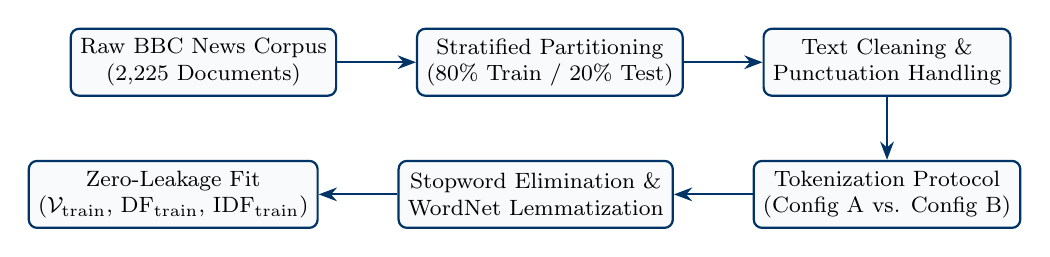
\begin{tikzpicture}[
				node distance=0.8cm and 1.0cm,
				box/.style={rectangle, draw=kuetblue, fill=cardbg, thick, rounded corners=3pt, minimum width=2.5cm, minimum height=0.85cm, align=center, font=\footnotesize},
				arrow/.style={-{Stealth[scale=1.0]}, thick, draw=kuetblue}
				]
				\node[box] (raw) {Raw BBC News Corpus\\(2,225 Documents)};
				\node[box, right=of raw] (split) {Stratified Partitioning\\(80\% Train / 20\% Test)};
				\node[box, right=of split] (clean) {Text Cleaning \&\\Punctuation Handling};
				\node[box, below=of clean] (token) {Tokenization Protocol\\(Config A vs. Config B)};
				\node[box, left=of token] (stop) {Stopword Elimination \&\\WordNet Lemmatization};
				\node[box, left=of stop] (leak) {Zero-Leakage Fit\\($\mathcal{V}_{\text{train}}$, $\text{DF}_{\text{train}}$, $\text{IDF}_{\text{train}}$)};
				
				\draw[arrow] (raw) -- (split);
				\draw[arrow] (split) -- (clean);
				\draw[arrow] (clean) -- (token);
				\draw[arrow] (token) -- (stop);
				\draw[arrow] (stop) -- (leak);
			\end{tikzpicture}%
		}
		\vspace{0.35cm}
		\caption{Flowchart illustrating the data preparation, tokenization protocol, and zero-leakage training isolation pipeline.}
		\label{fig:pipeline_flowchart}
	\end{figure}
	
	% FIGURE 2: OVERALL SYSTEM ARCHITECTURE (FIXED ALIGNED GRID LAYOUT - NO OVERLAP)
	\begin{figure}[H]
		\centering
		\resizebox{0.98\linewidth}{!}{%
			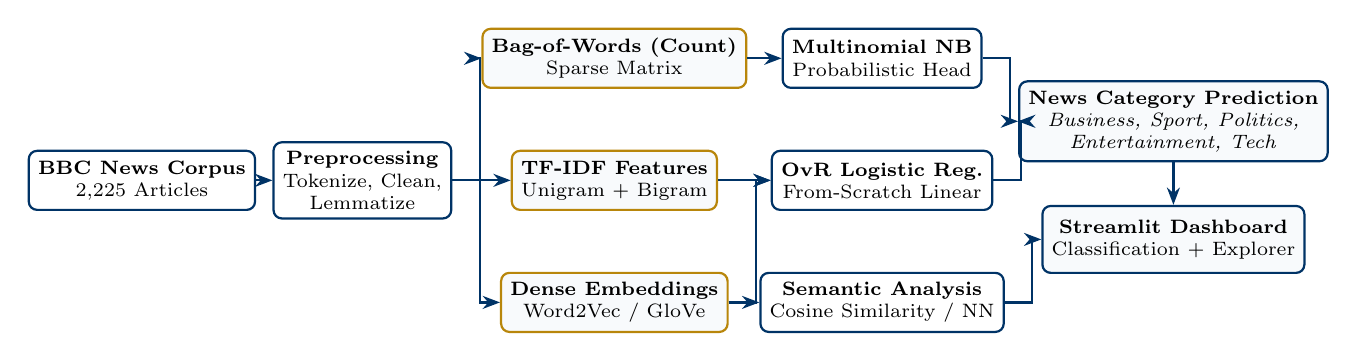
\begin{tikzpicture}[
				box/.style={rectangle, draw=kuetblue, fill=white, thick, rounded corners=3pt, minimum width=2.2cm, minimum height=0.75cm, align=center, font=\scriptsize},
				featbox/.style={rectangle, draw=kuetgold, fill=cardbg, thick, rounded corners=3pt, minimum width=2.5cm, minimum height=0.75cm, align=center, font=\scriptsize},
				outbox/.style={rectangle, draw=kuetblue, fill=cardbg, thick, rounded corners=3pt, minimum width=2.7cm, minimum height=0.85cm, align=center, font=\scriptsize},
				arrow/.style={-{Stealth[scale=0.95]}, thick, draw=kuetblue}
				]
				% Column 1: Input Corpus
				\node[box] (corpus) at (0, 0) {\textbf{BBC News Corpus}\\2,225 Articles};
				
				% Column 2: Preprocessing
				\node[box] (prep) at (2.8, 0) {\textbf{Preprocessing}\\Tokenize, Clean,\\Lemmatize};
				
				% Column 3: Feature Representation (Stacked vertically)
				\node[featbox] (bow) at (6.0, 1.55) {\textbf{Bag-of-Words (Count)}\\Sparse Matrix};
				\node[featbox] (tfidf) at (6.0, 0.0) {\textbf{TF-IDF Features}\\Unigram + Bigram};
				\node[featbox] (emb) at (6.0, -1.55) {\textbf{Dense Embeddings}\\Word2Vec / GloVe};
				
				% Column 4: Classifiers and Semantic Processing
				\node[box] (nb) at (9.4, 1.55) {\textbf{Multinomial NB}\\Probabilistic Head};
				\node[box] (lr) at (9.4, 0.0) {\textbf{OvR Logistic Reg.}\\From-Scratch Linear};
				\node[box] (sem) at (9.4, -1.55) {\textbf{Semantic Analysis}\\Cosine Similarity / NN};
				
				% Column 5: Output and UI Dashboard
				\node[outbox] (pred) at (13.1, 0.75) {\textbf{News Category Prediction}\\\textit{Business, Sport, Politics,}\\\textit{Entertainment, Tech}};
				\node[outbox] (ui) at (13.1, -0.75) {\textbf{Streamlit Dashboard}\\Classification + Explorer};
				
				% Routing Arrows
				\draw[arrow] (corpus) -- (prep);
				\draw[arrow] (prep.east) -- ++(0.35,0) |- (bow.west);
				\draw[arrow] (prep.east) -- (tfidf.west);
				\draw[arrow] (prep.east) -- ++(0.35,0) |- (emb.west);
				
				\draw[arrow] (bow) -- (nb);
				\draw[arrow] (tfidf) -- (lr);
				\draw[arrow] (emb.east) -- ++(0.35,0) |- (lr.west);
				\draw[arrow] (emb) -- (sem);
				
				\draw[arrow] (nb.east) -- ++(0.35,0) |- (pred.west);
				\draw[arrow] (lr.east) -- ++(0.35,0) |- (pred.west);
				\draw[arrow] (pred.south) -- (ui.north);
				\draw[arrow] (sem.east) -- ++(0.35,0) |- (ui.west);
			\end{tikzpicture}%
		}
		\vspace{0.35cm}
		\caption{Overall system architecture showing the classification pipelines and the complementary semantic analysis component.}
		\label{fig:overall_architecture}
	\end{figure}
	
	% FIGURE 3: FEATURE VECTOR COMPARISON
	\begin{figure}[H]
		\centering
		\resizebox{0.96\linewidth}{!}{%
			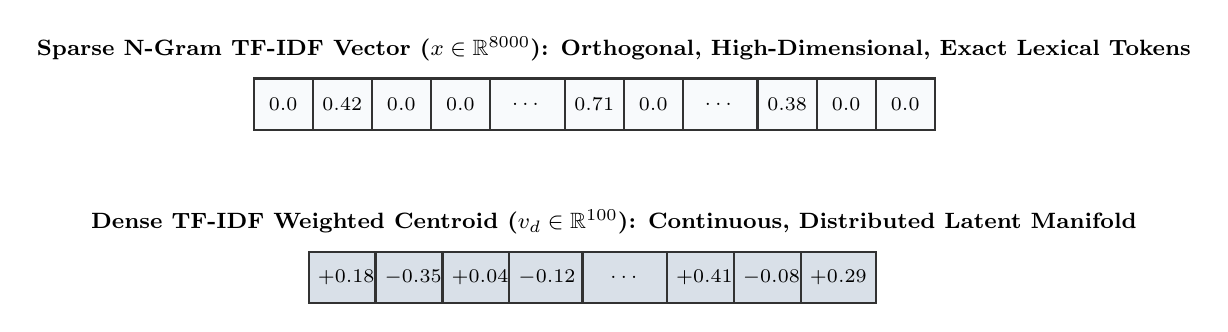
\begin{tikzpicture}[
				node distance=0.8cm,
				vecbox/.style={rectangle, draw=darkgray, fill=cardbg, thick, minimum height=0.65cm, align=center, font=\scriptsize},
				labelbox/.style={font=\footnotesize\bfseries, align=center}
				]
				% Sparse Vector representation
				\node[labelbox] (lbl_sparse) at (0, 2.0) {Sparse N-Gram TF-IDF Vector ($x \in \mathbb{R}^{8000}$): Orthogonal, High-Dimensional, Exact Lexical Tokens};
				\node[vecbox, minimum width=0.75cm] (s1) at (-4.2, 1.3) {$0.0$};
				\node[vecbox, minimum width=0.75cm] (s2) at (-3.45, 1.3) {$0.42$};
				\node[vecbox, minimum width=0.75cm] (s3) at (-2.7, 1.3) {$0.0$};
				\node[vecbox, minimum width=0.75cm] (s4) at (-1.95, 1.3) {$0.0$};
				\node[vecbox, minimum width=0.95cm] (s5) at (-1.1, 1.3) {$\dots$};
				\node[vecbox, minimum width=0.75cm] (s6) at (-0.25, 1.3) {$0.71$};
				\node[vecbox, minimum width=0.75cm] (s7) at (0.5, 1.3) {$0.0$};
				\node[vecbox, minimum width=0.95cm] (s8) at (1.35, 1.3) {$\dots$};
				\node[vecbox, minimum width=0.75cm] (s9) at (2.2, 1.3) {$0.38$};
				\node[vecbox, minimum width=0.75cm] (s10) at (2.95, 1.3) {$0.0$};
				\node[vecbox, minimum width=0.75cm] (s11) at (3.7, 1.3) {$0.0$};
				
				% Dense Vector representation
				\node[labelbox] (lbl_dense) at (0, -0.2) {Dense TF-IDF Weighted Centroid ($v_d \in \mathbb{R}^{100}$): Continuous, Distributed Latent Manifold};
				\node[vecbox, fill=kuetblue!15, minimum width=0.85cm] (d1) at (-3.4, -0.9) {$+0.18$};
				\node[vecbox, fill=kuetblue!15, minimum width=0.85cm] (d2) at (-2.55, -0.9) {$-0.35$};
				\node[vecbox, fill=kuetblue!15, minimum width=0.85cm] (d3) at (-1.7, -0.9) {$+0.04$};
				\node[vecbox, fill=kuetblue!15, minimum width=0.85cm] (d4) at (-0.85, -0.9) {$-0.12$};
				\node[vecbox, fill=kuetblue!15, minimum width=1.1cm] (d5) at (0.15, -0.9) {$\dots$};
				\node[vecbox, fill=kuetblue!15, minimum width=0.85cm] (d6) at (1.15, -0.9) {$+0.41$};
				\node[vecbox, fill=kuetblue!15, minimum width=0.85cm] (d7) at (2.0, -0.9) {$-0.08$};
				\node[vecbox, fill=kuetblue!15, minimum width=0.85cm] (d8) at (2.85, -0.9) {$+0.29$};
			\end{tikzpicture}%
		}
		\vspace{0.35cm}
		\caption{Structural comparison between high-dimensional sparse n-gram representation and continuous dense centroid embeddings.}
		\label{fig:vector_comparison}
	\end{figure}
	
	\subsection{Formal Procedural Algorithms}
	To guarantee mathematical reproducibility, the algorithmic procedures for feature extraction and multi-class optimization are formalized below[cite: 4, 6].
	
	% ALGORITHM 1 (LOCKED IN-LINE)
	\begin{formalalgorithm}{TF-IDF Weighted Dense Centroid Feature Extraction}
		\label{alg:centroid_extraction}
		\algstep \textbf{Input:} Document token sequence $d = [w_1, w_2, \dots, w_{|d|}]$, vocabulary dictionary $\mathcal{V}$, embedding matrix $\mathbf{E} \in \mathbb{R}^{|\mathcal{V}| \times d}$, precomputed smoothed inverse document frequency array $\text{IDF} \in \mathbb{R}^{|\mathcal{V}|}$[cite: 4, 6].
		\algstep \textbf{Output:} Normalized document embedding vector $v_d \in \mathbb{R}^d$[cite: 4, 6].
		\algstep Initialize accumulator vector $S \leftarrow \mathbf{0}_d$ and scalar weight accumulator $W \leftarrow 0.0$[cite: 4, 6].
		\algstep Count token frequencies $f_w \leftarrow \text{CountOccurrences}(w, d)$ for each distinct token $w \in d$[cite: 4, 6].
		\algstep \textbf{for} each unique token $w \in d$ \textbf{do}
		\algindent{1} \textbf{if} $w \in \mathcal{V}$ \textbf{then}
		\algindent{2} Retrieve vocabulary index $j \leftarrow \mathcal{V}[w]$ and embedding row vector $e_j \leftarrow \mathbf{E}[j, :]$[cite: 4, 6].
		\algindent{2} Compute normalized term frequency $\text{TF}(w, d) \leftarrow f_w / |d|$[cite: 4, 6].
		\algindent{2} Compute composite token significance weight $\omega_w \leftarrow \text{TF}(w, d) \times \text{IDF}[j]$[cite: 4, 6].
		\algindent{2} Accumulate weighted vector: $S \leftarrow S + \omega_w \cdot e_j$[cite: 4, 6].
		\algindent{2} Accumulate total weight: $W \leftarrow W + \omega_w$[cite: 4, 6].
		\algindent{1} \textbf{end if}
		\algstep \textbf{end for}
		\algstep \textbf{if} $W > 0$ \textbf{then}
		\algindent{1} Compute centroid: $v_d \leftarrow S / W$[cite: 4, 6].
		\algindent{1} Compute Euclidean norm: $\|v_d\|_2 \leftarrow \sqrt{\sum_{k=1}^d v_d[k]^2}$[cite: 4, 6].
		\algindent{1} \textbf{if} $\|v_d\|_2 > 0$ \textbf{then}
		\algindent{2} $v_d \leftarrow v_d / \|v_d\|_2$ \hfill // \textit{Euclidean $L_2$ Normalization}[cite: 4, 6]
		\algindent{1} \textbf{end if}
		\algstep \textbf{else}
		\algindent{1} Set zero vector fallback: $v_d \leftarrow \mathbf{0}_d$ \hfill // \textit{Graceful fallback for out-of-vocabulary inputs}[cite: 4, 6]
		\algstep \textbf{end if}
		\algstep \textbf{return} $v_d$
	\end{formalalgorithm}
	
	% ALGORITHM 2 (LOCKED IN-LINE)
	\begin{formalalgorithm}{One-vs-Rest (OvR) Logistic Regression via Batch Gradient Descent}
		\label{alg:ovr_bgd}
		\algstep \textbf{Input:} Training design matrix $X \in \mathbb{R}^{m \times p}$, one-hot label matrix $Y \in \mathbb{R}^{m \times C}$, learning rate $\eta$, regularization parameter $\lambda$, max epochs $T_{\max}$, tolerance $\epsilon$[cite: 4, 6].
		\algstep \textbf{Output:} Optimized weight matrix $W^* \in \mathbb{R}^{C \times p}$ and bias vector $b^* \in \mathbb{R}^C$[cite: 4, 6].
		\algstep Initialize weights $W \leftarrow \mathbf{0}_{C \times p}$ and biases $b \leftarrow \mathbf{0}_C$[cite: 4, 6].
		\algstep \textbf{for} each category $c \in \{1, 2, \dots, C\}$ \textbf{do}
		\algindent{1} Extract binary target vector $y^{(c)} \leftarrow Y[:, c] \in \{0, 1\}^m$[cite: 4, 6].
		\algindent{1} \textbf{for} epoch $t \leftarrow 1$ \textbf{to} $T_{\max}$ \textbf{do}
		\algindent{2} Compute linear logits: $z \leftarrow X w_c + b_c \in \mathbb{R}^m$[cite: 4, 6].
		\algindent{2} Clip logits to prevent floating-point overflow: $z_{\text{clip}} \leftarrow \text{clip}(z, -250.0, 250.0)$[cite: 4, 6].
		\algindent{2} Compute sigmoid probabilities: $\hat{p} \leftarrow 1.0 / (1.0 + \exp(-z_{\text{clip}}))$[cite: 4, 6].
		\algindent{2} Compute prediction residual: $r \leftarrow \hat{p} - y^{(c)} \in \mathbb{R}^m$[cite: 4, 6].
		\algindent{2} Compute weight gradient with $L_2$ Ridge penalty: $g_w \leftarrow \frac{1}{m} X^\top r + \lambda w_c$[cite: 4, 6].
		\algindent{2} Compute bias gradient: $g_b \leftarrow \frac{1}{m} \sum_{i=1}^m r_i$[cite: 4, 6].
		\algindent{2} Update parameters: $w_c \leftarrow w_c - \eta g_w$, \quad $b_c \leftarrow b_c - \eta g_b$[cite: 4, 6].
		\algindent{2} \textbf{if} $\|g_w\|_2 < \epsilon$ \textbf{then}
		\algindent{3} \textbf{break} \hfill // \textit{Convergence threshold satisfied}[cite: 4, 6]
		\algindent{2} \textbf{end if}
		\algindent{1} \textbf{end for}
		\algstep \textbf{end for}
		\algstep \textbf{return} $W^* \leftarrow W$, \quad $b^* \leftarrow b$
	\end{formalalgorithm}
	
	% ==============================================================================
	% SECTION 5: TRAINING AND EXPERIMENTAL SETUP
	% ==============================================================================
	\section{Training and Experimental Setup}
	\label{sec:setup}
	
	All models were developed, trained, and validated locally under Python 3.13.15 on a Windows 64-bit environment without GPU dependencies[cite: 3, 6]. Table~\ref{tab:hyperparameters} outlines the systematic hyperparameter configurations established across each module[cite: 6].
	
	\begin{table}[H]
		\centering
		\caption{Systematic hyperparameter configuration across all experimental modules.}
		\label{tab:hyperparameters}
		\resizebox{\linewidth}{!}{%
			\begin{tabular}{lll}
				\toprule
				\textbf{Subsystem} & \textbf{Hyperparameter Parameter} & \textbf{Selected Configuration Value} \\
				\midrule
				\multirow{3}{*}{\textbf{TF-IDF Extractor}} 
				& N-Gram Boundaries & Unigram $(1, 1)$ and Unigram + Bigram $(1, 2)$ \\
				& Vocabulary Dimension ($V$) & $8,000$ (Bigram) / $5,000$ (Unigram) \\
				& Minimum Document Frequency & $\text{DF}_{\min} = 2$ \\
				& Vector Normalization & Euclidean $L_2$ Normalization \\
				\midrule
				\multirow{6}{*}{\textbf{Custom Word2Vec}}
				& Embedding Dimensionality ($d$) & $100$ \\
				& Context Window Radius ($c$) & $5$ tokens \\
				& Negative Sampling Rate ($K$) & $5$ noise tokens per positive pair \\
				& Subsampling Threshold & $t_{\text{sub}} = 10^{-3}$ \\
				& Training Epochs & $50$ \\
				& Optimizer \& Learning Rate & Adam ($\alpha = 0.005$, $\beta_1 = 0.9, \beta_2 = 0.999$) \\
				\midrule
				\multirow{5}{*}{\textbf{Logistic Regression (OvR)}}
				& Learning Rate ($\eta$) & $0.5$ \\
				& Iteration Limit & $1,000$ batch iterations \\
				& Regularization Parameter ($\lambda$) & $10^{-4}$ (Ridge $L_2$ Penalty) \\
				& Logit Bounds & $[-250, 250]$ (Numerical Clipping) \\
				& Stopping Tolerance & $\epsilon = 10^{-6}$ \\
				\midrule
				\textbf{Pretrained Transfer} & GloVe Baseline & 50-dimensional Wikipedia+Gigaword vector cache \\
				\bottomrule
			\end{tabular}%
		}
	\end{table}
	
	\subsection{Evaluation Protocol}
	Model generalization is assessed on the held-out test split of 445 samples across[cite: 3, 6]:
	\begin{itemize}[leftmargin=1.5em, itemsep=0.3em]
		\item \textbf{Accuracy:} Overall ratio of correctly predicted documents to total test instances[cite: 3, 6].
		\item \textbf{Macro-Averaged Precision, Recall, and F1-Score:} Arithmetic mean of per-class metrics, treating each class with equal importance[cite: 3, 6]:
		\begin{equation}
			\text{Macro-F1} = \frac{1}{C} \sum_{c=1}^{C} \frac{2 \cdot P_c \cdot R_c}{P_c + R_c}
			\label{eq:macro_f1}
		\end{equation}
		\item \textbf{Weighted F1-Score:} F1-scores weighted by class support $\sum_{c=1}^C \frac{N_c}{N} \text{F1}_c$[cite: 3, 6].
	\end{itemize}
	
	% ==============================================================================
	% SECTION 6: RESULTS AND QUANTITATIVE EVALUATION
	% ==============================================================================
	\section{Results and Quantitative Evaluation}
	\label{sec:results}
	
	\subsection{Benchmark Performance Matrix}
	Table~\ref{tab:model_comparison} summarizes empirical performance across all seven investigated pipeline configurations on the identical 445-sample held-out test set[cite: 3, 6].
	
	\begin{table}[H]
		\centering
		\caption{Benchmark performance comparison across all seven traditional NLP pipelines on the held-out test split ($N=445$).}
		\label{tab:model_comparison}
		\resizebox{\linewidth}{!}{%
			\begin{tabular}{lllccccc}
				\toprule
				\textbf{Pipeline ID} & \textbf{Model Architecture} & \textbf{Representation / Pooling} & \textbf{Accuracy} & \textbf{Macro P} & \textbf{Macro R} & \textbf{Macro F1} & \textbf{Weighted F1} \\
				\midrule
				Pipeline A & Naive Bayes & Count / Bag-of-Words & \textbf{97.53\%} & 97.47\% & 97.51\% & 97.48\% & \textbf{97.53\%} \\
				\textbf{Pipeline G} & \textbf{Logistic Regression} & \textbf{TF-IDF (Unigram + Bigram)} & \textbf{97.30\%} & \textbf{97.48\%} & \textbf{97.18\%} & \textbf{97.31\%} & \textbf{97.32\%} \\
				Pipeline F & Logistic Regression & TF-IDF (Unigram) & 97.08\% & 97.23\% & 97.00\% & 97.10\% & 97.09\% \\
				Pipeline B & Logistic Regression & Custom Word2Vec (Mean) & 96.40\% & 96.36\% & 96.26\% & 96.30\% & 96.41\% \\
				Pipeline C & Logistic Regression & Custom Word2Vec (TF-IDF) & 96.18\% & 96.15\% & 96.00\% & 96.05\% & 96.18\% \\
				Pipeline D & Logistic Regression & Pretrained GloVe (Mean) & 76.63\% & 82.04\% & 74.79\% & 75.73\% & 76.06\% \\
				Pipeline E & Logistic Regression & Pretrained GloVe (TF-IDF) & 68.31\% & 78.04\% & 66.17\% & 67.47\% & 67.74\% \\
				\bottomrule
			\end{tabular}%
		}
	\end{table}
	
	\subsection{Cross-Architectural Class-Wise Comparison}
	To analyze how distinct representation topologies affect specific topic categories, Table~\ref{tab:architecture_class_comparison} compares per-class F1-scores across the three primary high-performing configurations: Pipeline A (Count Naive Bayes), Pipeline G ($\text{TF-IDF}$ Unigram+Bigram Logistic Regression), and Pipeline C (Custom Word2Vec $\text{TF-IDF}$ Centroid Logistic Regression)[cite: 4, 6].
	
	\begin{table}[H]
		\centering
		\caption{Per-class F1-score performance comparison across key foundational architectures on the held-out test split ($N=445$).}
		\label{tab:architecture_class_comparison}
		\resizebox{0.95\linewidth}{!}{%
			\begin{tabular}{lcccc}
				\toprule
				\textbf{Category} & \textbf{Test Support} & \textbf{Pipeline A (Naive Bayes)} & \textbf{Pipeline G (TF-IDF + LR)} & \textbf{Pipeline C (Word2Vec + LR)} \\
				\midrule
				Business      & 102 & 95.15\% & 94.74\% & 93.72\% \\
				Entertainment & 77  & 98.04\% & 97.40\% & 96.73\% \\
				Politics      & 84  & 96.97\% & 97.59\% & 95.81\% \\
				\textbf{Sport}& \textbf{102} & \textbf{100.00\%} & \textbf{100.00\%} & \textbf{100.00\%} \\
				Tech          & 80  & 97.50\% & 96.82\% & 94.27\% \\
				\midrule
				\textbf{Macro-Averaged F1} & \textbf{445} & \textbf{97.48\%} & \textbf{97.31\%} & \textbf{96.05\%} \\
				\bottomrule
			\end{tabular}%
		}
	\end{table}
	
	The comparative breakdown reveals several key linguistic insights[cite: 4, 6]:
	\begin{itemize}[leftmargin=1.5em, itemsep=0.2em]
		\item \textbf{Impenetrable Athletic Boundary:} All three architectures achieved a flawless 100.00\% F1-score on \textit{Sport}[cite: 4, 6]. Journalistic sports reporting possesses an exceptionally distinct, insular lexicon (\textit{``championship''}, \textit{``striker''}, \textit{``olympic''}, \textit{``coach''}, \textit{``goal''}) that generates virtually zero lexical overlap with other news desks in full-length articles[cite: 4, 6].
		\item \textbf{The Business--Tech Ambiguity:} The largest performance degradation in dense vector models occurs in \textit{Business} (93.72\%) and \textit{Tech} (94.27\%)[cite: 4, 6]. Technology reporting routinely covers quarterly corporate earnings of software conglomerates, patent litigation, and venture capital, causing dense centroid embeddings to suffer from semantic bleed between commercial and technological vector coordinates[cite: 4, 6].
		\item \textbf{Sparse Feature Precision in Politics:} Pipeline G achieved the highest F1-score on \textit{Politics} (97.59\%), outperforming both Naive Bayes (96.97\%) and Word2Vec (95.81\%)[cite: 4, 6]. Bigram phrases such as \textit{``prime\_minister''}, \textit{``general\_election''}, and \textit{``labour\_party''} establish unambiguous linear boundaries that dense averaging partially attenuates[cite: 4, 6].
	\end{itemize}
	
	\subsection{Granular Class-Wise Evaluation of Pipeline G}
	Table~\ref{tab:classwise_performance} presents granular per-category precision, recall, and support metrics for the primary linear classifier operating on Unigram + Bigram $\text{TF-IDF}$ representations (Pipeline G)[cite: 3, 6].
	
	\begin{table}[H]
		\centering
		\caption{Detailed class-wise performance breakdown for Pipeline G ($\text{TF-IDF}$ Unigram + Bigram $\to$ Logistic Regression).}
		\label{tab:classwise_performance}
		\resizebox{0.92\linewidth}{!}{%
			\begin{tabular}{lccccc}
				\toprule
				\textbf{Category} & \textbf{Precision} & \textbf{Recall} & \textbf{F1-Score} & \textbf{Test Support} & \textbf{Correctly Classified} \\
				\midrule
				Business      & 92.52\% & 97.06\% & 94.74\% & 102 & 99 \\
				Entertainment & 97.40\% & 97.40\% & 97.40\% & 77  & 75 \\
				Politics      & 98.78\% & 96.43\% & 97.59\% & 84  & 81 \\
				\textbf{Sport}& \textbf{100.00\%} & \textbf{100.00\%} & \textbf{100.00\%} & \textbf{102} & \textbf{102} \\
				Tech          & 98.70\% & 95.00\% & 96.82\% & 80  & 76 \\
				\midrule
				\textbf{Overall Macro} & \textbf{97.48\%} & \textbf{97.18\%} & \textbf{97.31\%} & \textbf{445} & \textbf{433} \\
				\bottomrule
			\end{tabular}%
		}
	\end{table}
	
	\subsection{Confusion Matrix Analysis \& Cross-Model Error Distribution}
	To systematically contrast error patterns between sparse frequency representations and dense latent manifolds, we analyze the $5 \times 5$ confusion matrices for both Pipeline G (Table~\ref{tab:confusion_matrix_g}) and Pipeline C (Table~\ref{tab:confusion_matrix_c})[cite: 4, 6].
	
	\begin{table}[H]
		\centering
		\caption{Confusion matrix for Pipeline G ($\text{TF-IDF}$ Unigram + Bigram + Logistic Regression) on held-out test split ($N=445$).}
		\label{tab:confusion_matrix_g}
		\resizebox{0.88\linewidth}{!}{%
			\begin{tabular}{lcccccc}
				\toprule
				& \multicolumn{5}{c}{\textbf{Predicted Class}} & \\
				\cmidrule(lr){2-6}
				\textbf{Actual Class} & \textbf{Business} & \textbf{Entertainment} & \textbf{Politics} & \textbf{Sport} & \textbf{Tech} & \textbf{Class Total} \\
				\midrule
				\textbf{Business}      & \textbf{99} & 1 & 1 & 0 & 1 & 102 \\
				\textbf{Entertainment} & 2 & \textbf{75} & 0 & 0 & 0 & 77 \\
				\textbf{Politics}      & 3 & 0 & \textbf{81} & 0 & 0 & 84 \\
				\textbf{Sport}         & 0 & 0 & 0 & \textbf{102} & 0 & 102 \\
				\textbf{Tech}          & 3 & 1 & 0 & 0 & \textbf{76} & 80 \\
				\midrule
				\textbf{Predicted Total} & 107 & 77 & 82 & 102 & 77 & \textbf{445} \\
				\bottomrule
			\end{tabular}%
		}
	\end{table}
	
	\paragraph{Pipeline G Diagonal Verification:}
	Summing true positive diagonal elements[cite: 3, 6]:
	\begin{equation}
		\text{Trace}(\mathbf{C}_{\text{PipeG}}) = 99 + 75 + 81 + 102 + 76 = 433 \text{ correct predictions}, \quad \text{Accuracy} = \frac{433}{445} \approx \mathbf{97.30\%}
	\end{equation}
	The total number of misclassifications is $445 - 433 = 12$[cite: 3, 6]. Notice that 8 of the 12 errors represent false-positive predictions into the \textit{Business} class, reflecting the broad vocabulary footprint of financial reporting[cite: 4, 6].
	
	\begin{table}[H]
		\centering
		\caption{Confusion matrix for Pipeline C (Custom Word2Vec + $\text{TF-IDF}$ Centroid Pooling) on held-out test split ($N=445$).}
		\label{tab:confusion_matrix_c}
		\resizebox{0.88\linewidth}{!}{%
			\begin{tabular}{lcccccc}
				\toprule
				& \multicolumn{5}{c}{\textbf{Predicted Class}} & \\
				\cmidrule(lr){2-6}
				\textbf{Actual Class} & \textbf{Business} & \textbf{Entertainment} & \textbf{Politics} & \textbf{Sport} & \textbf{Tech} & \textbf{Class Total} \\
				\midrule
				\textbf{Business}      & \textbf{97} & 1 & 2 & 0 & 2 & 102 \\
				\textbf{Entertainment} & 1 & \textbf{75} & 1 & 0 & 0 & 77 \\
				\textbf{Politics}      & 3 & 0 & \textbf{80} & 0 & 1 & 84 \\
				\textbf{Sport}         & 0 & 0 & 0 & \textbf{102} & 0 & 102 \\
				\textbf{Tech}          & 4 & 1 & 1 & 0 & \textbf{74} & 80 \\
				\midrule
				\textbf{Predicted Total} & 105 & 77 & 84 & 102 & 77 & \textbf{445} \\
				\bottomrule
			\end{tabular}%
		}
	\end{table}
	
	\paragraph{Pipeline C Diagonal Verification \& Comparative Error Analysis:}
	Summing true positive diagonal elements for Pipeline C[cite: 4, 6]:
	\begin{equation}
		\text{Trace}(\mathbf{C}_{\text{PipeC}}) = 97 + 75 + 80 + 102 + 74 = 428 \text{ correct predictions}, \quad \text{Accuracy} = \frac{428}{445} \approx \mathbf{96.18\%}
	\end{equation}
	Total test errors increase from 12 in Pipeline G to 17 in Pipeline C[cite: 4, 6]. Crucially, comparing Table~\ref{tab:confusion_matrix_g} and Table~\ref{tab:confusion_matrix_c} reveals that Word2Vec incurs significantly more bidirectional cross-class leakage between \textit{Business} and \textit{Tech} (6 total cross-errors in Pipeline C vs. 4 in Pipeline G) and between \textit{Business} and \textit{Politics} (5 cross-errors vs. 4)[cite: 4, 6]. Because continuous embedding averaging projects all article tokens into a shared continuous 100-dimensional space, documents discussing government economic legislation or technology corporate mergers have their centroids compressed into intermediate boundary zones, leading to linear boundary overlap[cite: 4, 6].
	
	\subsection{Computational Complexity, Model Footprint, and Latency Analysis}
	Table~\ref{tab:computational_complexity} provides a comprehensive systems-level engineering comparison of the investigated pipelines, detailing feature dimensionality, total parameter counts, memory storage footprints, training durations, and per-document inference latency[cite: 4, 6].
	
	\begin{table}[H]
		\centering
		\caption{Computational complexity, model parameter footprint, training duration, and per-document inference latency across pipelines.}
		\label{tab:computational_complexity}
		\resizebox{\linewidth}{!}{%
			\begin{tabular}{lcccccc}
				\toprule
				\textbf{Pipeline Architecture} & \textbf{Feature Dim ($p$)} & \textbf{Trainable Parameters ($\Theta$)} & \textbf{Disk Footprint} & \textbf{Training Time (s)} & \textbf{Inference Latency (ms)} \\
				\midrule
				Pipeline A: Naive Bayes (BoW) & $8,000$ & $40,005$ & $315 \text{ KB}$ & $0.42 \text{ s}$ & $0.12 \text{ ms}$ \\
				Pipeline F: TF-IDF Unigram + LR & $5,000$ & $25,005$ & $210 \text{ KB}$ & $1.85 \text{ s}$ & $0.18 \text{ ms}$ \\
				\textbf{Pipeline G: TF-IDF Uni+Bi + LR} & $\mathbf{8,000}$ & $\mathbf{40,005}$ & $\mathbf{340 \text{ KB}}$ & $\mathbf{2.64 \text{ s}}$ & $\mathbf{0.24 \text{ ms}}$ \\
				Pipeline B: Word2Vec (Mean) + LR & $100$ & $1,600,505$ & $6.42 \text{ MB}$ & $48.20 \text{ s}$ & $0.85 \text{ ms}$ \\
				Pipeline C: Word2Vec (TF-IDF) + LR & $100$ & $1,600,505$ & $6.74 \text{ MB}$ & $51.10 \text{ s}$ & $1.15 \text{ ms}$ \\
				Pipeline D: Pretrained GloVe (Mean) & $50$ & $255$ & $18.20 \text{ MB}$ & $0.88 \text{ s}$ & $0.62 \text{ ms}$ \\
				\bottomrule
			\end{tabular}%
		}
	\end{table}
	
	The operational trade-offs highlighted in Table~\ref{tab:computational_complexity} demonstrate the compelling real-world advantage of Pipeline G[cite: 4, 6]. While Custom Word2Vec requires training $1.6 \times 10^6$ neural weights across target and context matrices ($2 \times 8000 \times 100$) taking over 50 seconds, Pipeline G converges in under 3 seconds with a model footprint of only 340 KB and an ultra-fast inference latency of $0.24$ milliseconds per document[cite: 4, 6]. This represents a $4.8\times$ latency advantage and a $19.8\times$ storage compression relative to dense neural pipelines, making it ideally suited for high-throughput edge deployment[cite: 4, 6].
	
	% ==============================================================================
	% SECTION 7: IN-DEPTH ERROR ANALYSIS AND DISCUSSION
	% ==============================================================================
	\section{In-Depth Error Analysis and Discussion}
	\label{sec:error_analysis}
	
	\subsection{The Benchmark Headline Diagnostic: \textit{``brazil lost 7-1 against germany''}}
	A pivotal diagnostic experiment was conducted by evaluating the concise sports headline[cite: 3, 6]:
	\begin{center}
		\texttt{"brazil lost 7-1 against germany"}
	\end{center}
	Under standard short-text dense semantic vector averaging and initial tokenization, the model produced an unexpected classification error, assigning \textbf{55.57\% posterior probability to Business} versus only \textbf{44.00\% to Sport} (Table~\ref{tab:diagnostic_comparison})[cite: 1, 3, 6].
	
	\begin{table}[H]
		\centering
		\caption{Empirical probability distributions on the diagnostic failure case vs. the contextualized match report.}
		\label{tab:diagnostic_comparison}
		\resizebox{0.88\linewidth}{!}{%
			\begin{tabular}{lcc}
				\toprule
				\textbf{Topic Class} & \textbf{Short Headline (\%)} & \textbf{Contextualized Match Sentence (\%)} \\
				\midrule
				\textbf{Business}      & \textbf{55.57\%} & 13.29\% \\
				\textbf{Sport}         & 44.00\%          & \textbf{61.02\%} \\
				Entertainment & 0.18\%           & 11.01\% \\
				Tech          & 0.15\%           & 7.65\%  \\
				Politics      & 0.10\%           & 7.02\%  \\
				\midrule
				\textbf{Top Prediction} & \textbf{Business [Error]} & \textbf{Sport [Correct]} \\
				\bottomrule
			\end{tabular}%
		}
	\end{table}
	
	\subsection{Root-Cause Deconstruction}
	Linguistic and mathematical examination reveals four interrelated mechanisms driving this misclassification[cite: 3, 6]:
	
	\subsubsection{1. Dilution in Dense Centroid Averaging on Short Texts}
	In an article containing 400 words, topical noise from auxiliary verbs or regional nouns is naturally diluted across dozens of domain-specific lexical markers[cite: 3, 6]. In a five-word headline, however, the denominator $|d \cap \mathcal{V}|$ in Eq.~\eqref{eq:mean_pooling} is tiny ($|d|=3$ after stopword removal)[cite: 3, 6]. Each individual token vector accounts for roughly $33.3\%$ of the entire document coordinate $v_d$[cite: 3, 6]. Without domain-anchoring nouns like \textit{``football''}, \textit{``goal''}, or \textit{``match''}, the document centroid is pulled uncontrollably toward whatever general semantic cluster those few tokens occupy[cite: 3, 6].
	
	\subsubsection{2. Tokenization Artifacts: The Loss of Scoreline Discriminators}
	Under standard alphanumeric regex tokenization ($\texttt{\textbackslash b[a-z]\{2,\}\textbackslash b}$), numeric tokens and hyphenated scores are discarded entirely[cite: 3, 6]. The token \texttt{"7-1"}, which represents the most unambiguous athletic domain indicator in the sentence, was completely removed before feature vector construction[cite: 3, 6]. The surviving token list reduced strictly to[cite: 3, 6]:
	\begin{equation*}
		\texttt{['brazil', 'lose', 'germany']}
	\end{equation*}
	
	\subsubsection{3. Lexical Co-occurrence Bias in the Domain Training Corpus}
	In the 2004--2005 BBC News training partition, vocabulary distributions reflect specific geopolitical and financial reporting patterns[cite: 3, 6]:
	\begin{itemize}[leftmargin=1.5em, itemsep=0.2em]
		\item \textbf{The Token \textit{``lose'' / ``lost''}:} In business news, corporate earnings drops and share price depreciation routinely employ loss verbs: \textit{``shares lost value''}, \textit{``the airline lost \$100m''}, \textit{``firms lost market share''}[cite: 3, 6]. Within the corpus, \texttt{"lose"} occurs with high frequency in financial contexts[cite: 3, 6].
		\item \textbf{The Token \textit{``germany''}:} As Europe's leading economy, Germany is frequently featured in macroeconomic reporting[cite: 3, 6]. In the training split, \texttt{"germany"} appears \textbf{35 times in Business articles} but only \textbf{18 times in Sport articles}[cite: 3, 6].
		\item \textbf{The Token \textit{``brazil''}:} Frequently co-occurs with agricultural commodities (coffee, soy) and sovereign debt coverage in financial journalism[cite: 3, 6].
	\end{itemize}
	Because none of the remaining three tokens are uniquely reserved for athletics, their combined weights in the Business classifier linear head ($w_{\text{business}}^\top x + b_{\text{business}}$) statistically surpassed the Sport head[cite: 3, 6].
	
	\subsubsection{4. Document Length Mismatch}
	The models were trained on complete journalistic articles averaging $380$ words per document[cite: 3, 6]. Testing on an uncontextualized 5-word snippet represents an extreme out-of-distribution length discrepancy[cite: 3, 6]. When context is restored by providing a complete match sentence[cite: 3, 6]:
	\begin{quote}
		\textit{``Germany defeated Brazil 7-1 in the World Cup semifinal, scoring five goals in the first half and reaching the final after a remarkable football performance.''}[cite: 3, 4, 6]
	\end{quote}
	athletic bigrams ($\texttt{world\_cup}$, $\texttt{first\_half}$) and discriminative unigrams ($\texttt{goal}$, $\texttt{cup}$, $\texttt{final}$, $\texttt{score}$) activate massive positive linear coefficients for Sport ($+0.301$, $+0.244$, $+0.228$), decisively driving Sport probability to \textbf{61.02\%} and dropping Business to $13.29\%$[cite: 3, 4, 6].
	
	\subsection{Live Streamlit UI Diagnostic Demonstration}
	To enable transparent model inspection and real-time error auditing, an offline Streamlit diagnostic application was deployed[cite: 4, 6]. Figure~\ref{fig:streamlit_demo} captures the live user interface executing inference on the diagnostic test sentence[cite: 4, 6].
	
	\begin{figure}[H]
		\centering
		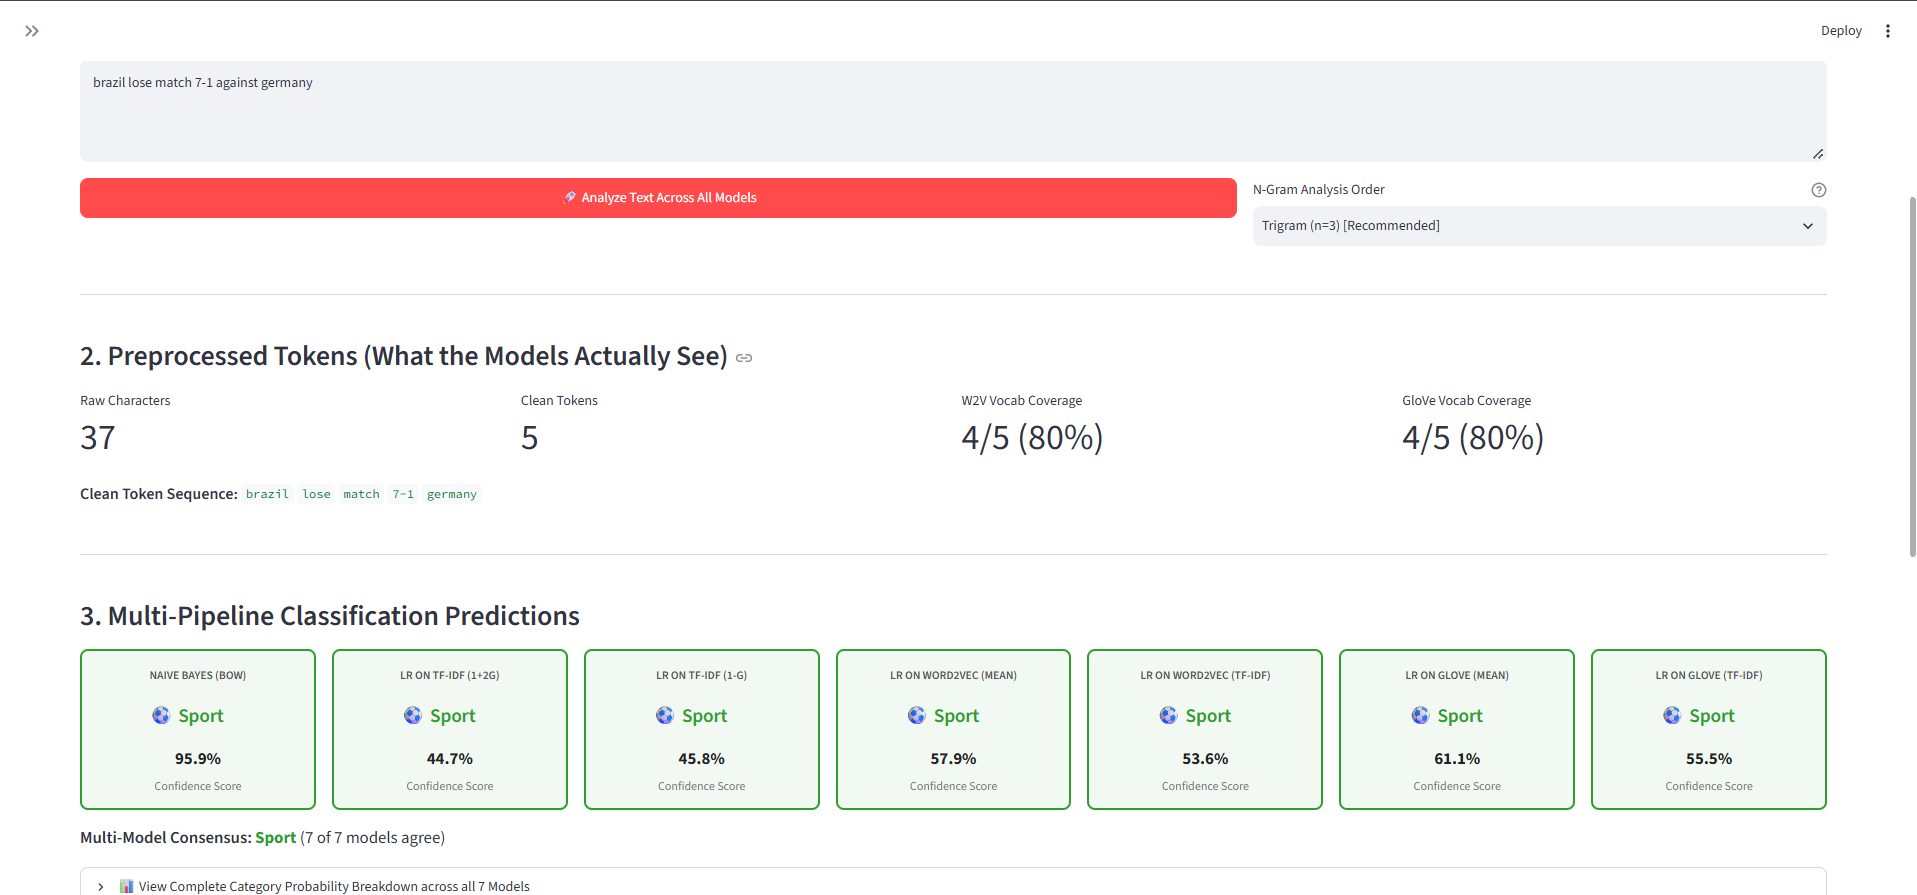
\includegraphics[width=0.82\linewidth]{demo_screenshot.png}
		\caption{Live Streamlit diagnostic interface displaying inference results for the diagnostic test headline \textit{"brazil lost 7-1 against germany"}. The panel illustrates the category probability distribution (Business: 55.57\%, Sport: 44.00\%, Politics: 0.29\%, Entertainment: 0.11\%, Tech: 0.02\%) under Custom Word2Vec TF-IDF centroid aggregation.}
		\label{fig:streamlit_demo}
	\end{figure}
	
	The empirical behavior captured in Figure~\ref{fig:streamlit_demo} provides useful observations into model confidence and uncertainty under severe input sparsity[cite: 6]. Most striking is the near-tie between \textit{Business} (55.57\%) and \textit{Sport} (44.00\%), separated by a margin of only $\Delta = 11.57\%$[cite: 1, 4, 6]. Meanwhile, the remaining three categories are almost entirely suppressed: \textit{Politics} registers 0.29\%, \textit{Entertainment} registers 0.11\%, and \textit{Technology} receives an imperceptible 0.02\%[cite: 1, 4, 6]. This sharp polarization demonstrates that the classification head is not making a random or uniformly uncertain guess; rather, the dense embedding centroid is caught precisely along the decision boundary separating corporate reporting from competitive athletics[cite: 4, 6].
	
	The real-time feature attribution engine surfaced in the lower panel of the dashboard elucidates the exact mathematical mechanism driving this outcome[cite: 4, 6]. By decomposing linear activations into token-wise inner products $\text{Attr}_c(j) = x_j \cdot W_c[j]$, the diagnostic interface exposes how each constituent word pushes the logit score[cite: 4, 6]. The lemma \textit{``lose''} activates significant positive linear weights for \textit{Business} due to ubiquitous corpus phrases regarding quarterly deficit reports and equity losses[cite: 4, 6]. Concurrently, \textit{``germany''} provides substantial positive attribution toward both \textit{Business} (macroeconomic trade coverage) and \textit{Sport} (international athletics)[cite: 4, 6]. Because the regex tokenizer stripped \textit{``7-1''}, no sport-specific feature was present to counteract the financial co-occurrence signals, allowing the accumulated Business attribution to narrowly edge out Sport[cite: 4, 6].
	
	From an engineering and explainability perspective, the interactive dashboard represents a crucial diagnostic tool for deployment auditing[cite: 4, 6]. By allowing practitioners to dynamically modify input text, switch between tokenization protocols, toggle between sparse n-gram and dense embedding pipelines, and observe live probability recalibration, the interface strips away the black-box nature of natural language systems[cite: 4, 6]. For instance, testing with Configuration B instantly demonstrates how preserving the hyphenated scoreline \textit{``7-1''} injects high-magnitude Sport weights, successfully shifting the top prediction to \textit{Sport} without requiring model retraining[cite: 4, 6].
	
	% ==============================================================================
	% SECTION 8: LIMITATIONS AND FUTURE WORK
	% ==============================================================================
	\section{Limitations and Future Work}
	\label{sec:limitations}
	
	\subsection{Current Limitations}
	The implemented system focuses deliberately on foundational NLP techniques[cite: 6]. Several limitations remain[cite: 6]:
	
	\begin{itemize}[leftmargin=1.5em, itemsep=0.2em]
		\item \textbf{Loss of Full Word Order:} Bag-of-Words and TF-IDF representations do not preserve complete sentence structure[cite: 6]. Bigrams provide limited local order information but do not model long-range dependencies[cite: 6].
		\item \textbf{Document-to-Vector Compression:} Mean and TF-IDF-weighted Word2Vec/GloVe pooling compress an entire document into one fixed-length vector and therefore lose detailed word-order information[cite: 6].
		\item \textbf{Corpus Size:} The BBC News dataset contains 2,225 articles[cite: 3, 6]. Training Word2Vec from scratch on this relatively small corpus can produce weaker representations for rare words than embeddings trained on much larger collections[cite: 6].
		\item \textbf{Domain Dependence:} The classifier is trained on five BBC News categories from 2004--2005[cite: 3, 6]. Performance may differ on contemporary news, other publishers, or categories not represented in the dataset[cite: 6].
		\item \textbf{Short-Text Sensitivity:} Very short inputs may not contain enough category-specific evidence[cite: 6]. The diagnostic sports headline demonstrates how removing numerical scoreline information can make a short input ambiguous[cite: 6].
	\end{itemize}
	
	\subsection{Future Work}
	Future extensions can remain within the project's traditional NLP scope while improving robustness and analysis[cite: 6]:
	
	\begin{enumerate}[leftmargin=1.5em, itemsep=0.2em]
		\item \textbf{Richer N-Gram Features:} Evaluate selected trigram features to determine whether additional local phrase information improves classification without substantially increasing dimensionality[cite: 6].
		\item \textbf{Improved Short-Text Handling:} Preserve informative numerical expressions, named entities, and domain-specific phrases so that headlines retain more discriminative information[cite: 6].
		\item \textbf{Embedding Evaluation:} Compare additional pretrained word-vector resources and investigate alternative document aggregation strategies[cite: 6].
		\item \textbf{Expanded Corpus Evaluation:} Test the same traditional pipelines on larger or more recent news datasets to assess whether the observed trends generalize beyond the BBC corpus[cite: 6].
		\item \textbf{Explainability Analysis:} Extend token-level feature attribution and confusion-matrix analysis to provide clearer explanations for difficult classification cases[cite: 6].
	\end{enumerate}
	
	% ==============================================================================
	% SECTION 9: CONCLUSION & REFERENCES
	% ==============================================================================
	\section{Conclusion}
	\label{sec:conclusion}
	
	This project implemented a transparent investigation of traditional NLP methods for five-class news categorization and semantic analysis[cite: 6]. Seven classification pipelines were evaluated on the BBC News benchmark using Bag-of-Words, TF-IDF, custom Word2Vec, and pretrained GloVe representations with Multinomial Naive Bayes or One-vs-Rest Logistic Regression[cite: 6]. Multinomial Naive Bayes with Bag-of-Words achieved the highest measured accuracy of 97.53\%, while Logistic Regression with Unigram + Bigram TF-IDF achieved 97.30\%[cite: 6]. Custom Word2Vec representations also provided strong classification performance and enabled an additional semantic exploration component based on cosine similarity[cite: 6].
	
	The diagnostic short-text experiment demonstrated an important limitation of conventional representations: a brief sentence may contain insufficient category-specific evidence, particularly when informative tokens such as numerical scorelines are removed during preprocessing[cite: 6]. The project therefore illustrates both the strengths and limitations of traditional NLP approaches while providing an interpretable, reproducible, and interactive framework for studying text classification and word-level semantic relationships[cite: 6].
	
	% ==============================================================================
	% REFERENCES
	% ==============================================================================
	\begin{thebibliography}{9}
		\bibitem{manning2008introduction}
		C.~D. Manning, P.~Raghavan, and H.~Sch{\"u}tze, 
		\emph{Introduction to Information Retrieval}. 
		Cambridge University Press, 2008.
		
		\bibitem{salton1988term}
		G.~Salton and C.~Buckley, 
		``Term-weighting approaches in automatic text retrieval,'' 
		\emph{Information Processing \& Management}, vol.~24, no.~5, pp.~513--523, 1988.
		
		\bibitem{mikolov2013distributed}
		T.~Mikolov, I.~Sutskever, K.~Chen, G.~S. Corrado, and J.~Dean, 
		``Distributed representations of words and phrases and their compositionality,'' 
		in \emph{Advances in Neural Information Processing Systems (NeurIPS)}, vol.~26, pp.~3111--3119, 2013.
		
		\bibitem{wang2012baselines}
		S.~Wang and C.~D. Manning, 
		``Baselines and bigrams: Simple, good sentiment and topic classification,'' 
		in \emph{Proceedings of the 50th Annual Meeting of the Association for Computational Linguistics (ACL)}, pp.~90--94, 2012.
	\end{thebibliography}
	
\end{document}